\documentclass[usenames,dvipsnames,tikz]{standalone}
\usetikzlibrary{shapes.geometric}
\usepackage{xcolor}
\colorlet{myBlue}{RoyalBlue!35!Cerulean}
\colorlet{myRed}{Red}
\usepackage{tikz}
\usepackage{standalone}
\begin{document}
	
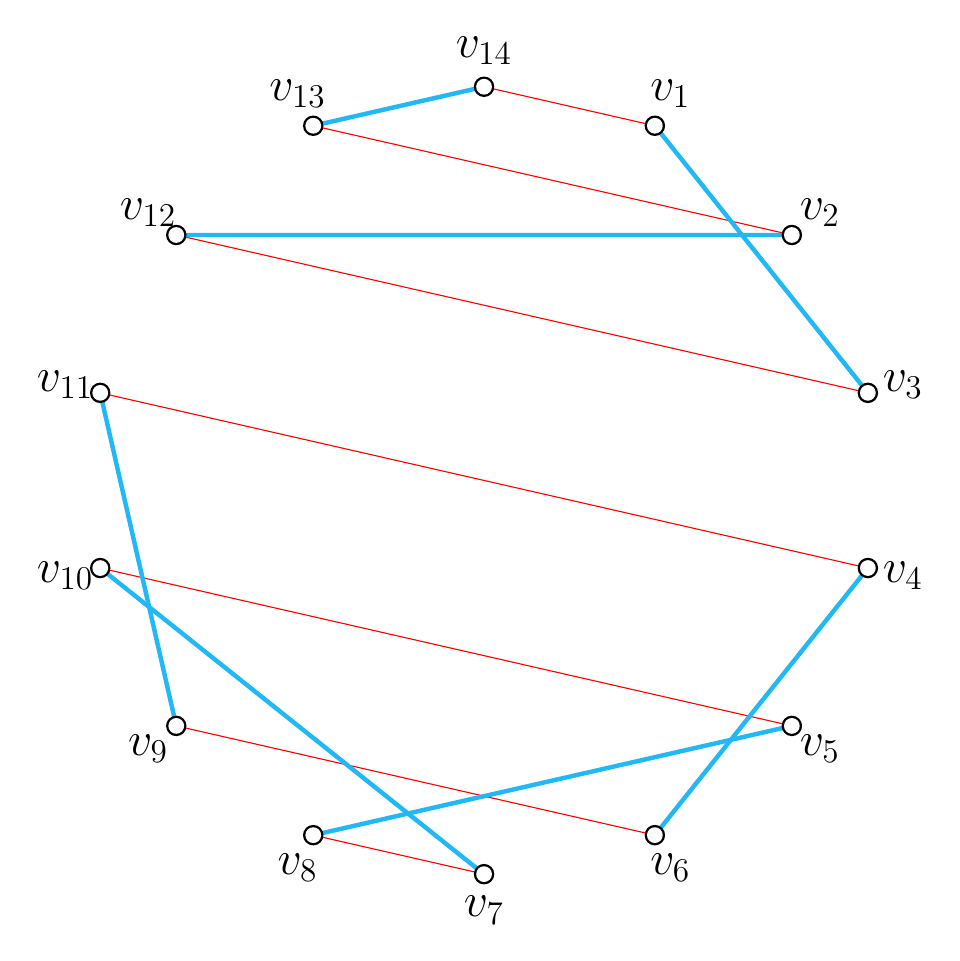
\begin{tikzpicture}
%Values of nodes:
% 1 = 1
% 2 = 1
% 3 = 2
% 4 = 2
% 5 = 2
% 6 = 3
% 7 = 3
% 8 = 4
% 9 = 4
% 10 = 5
% 11 = 5
% 12 = 6
% 13 = 7 (dominating)
% 14 = 7 (dominating)
% threshold tau = 7

\foreach \n/\value in {1/1, 2/1, 3/2, 4/2, 5/2, 6/3, 7/3, 8/4, 9/4, 10/5, 11/5, 12/6, 13/7, 14/7}
	\fill (90-\n*25.71428571:5cm) coordinate (v\n) circle [radius = 0.1]
		++(90-\n*25.71428571:13pt) node {\LARGE{$v_{\n}$}};
%		++(90-\n*25.71428571:18pt) node {\Large{(\value)}};
\foreach \m/\n in {1/14, 2/13, 3/12, 4/11, 5/10, 6/9, 7/8}
	\draw [myRed] (v\n) -- (v\m);
\foreach \m/\n in {1/3, 2/12, 4/6, 5/8, 7/10, 9/11, 13/14}
	\draw [ultra thick, myBlue] (v\n) -- (v\m);
\foreach \n in {1,...,14}
	\fill (90-\n*25.71428571:5cm) coordinate (v\n) circle [radius = 0.13];
\foreach \n in {1,...,14}
	\fill [white] (90-\n*25.71428571:5cm) coordinate (v\n) circle [radius = 0.1];

\end{tikzpicture}
	
\end{document}